\documentclass[
	a4paper, % Paper size, use either a4paper or letterpaper
	10pt, % Default font size, can also use 11pt or 12pt, although this is not recommended
	unnumberedsections, % Comment to enable section numbering
	twoside, % Two side traditional mode where headers and footers change between odd and even pages, comment this option to make them fixed
]{t0004}

\usepackage{xcolor}
\newcommand{\blue}[1]{\textcolor{blue}{#1}}
\newcommand{\gray}[1]{\textcolor{gray}{#1}}

\runninghead{Action Recognition YGAR} % A shortened article title to appear in the running head, leave this command empty for no running head

\setcounter{page}{1} % The page number of the first page, set this to a higher number if the article is to be part of an issue or larger work

%----------------------------------------------------------------------------------------
%	TITLE SECTION
%----------------------------------------------------------------------------------------

\title{Action Recognition\\ Utilizing YGAR Dataset} % Article title, use manual lines breaks (\\) to beautify the layout

\author{
	Shuo Wang, Amiya Ranjan and Lawrence Jiang
}

\date{\footnotesize DATASCI 281 Computer Vision \\ UC Berkeley School of Information \\ \{shuo.wang2, aranjan, lawrencejiang0797\}@berkeley.edu}

% Full-width abstract
\renewcommand{\maketitlehookd}{%
	\begin{abstract}
		\noindent placeholder
	\end{abstract}
}

%----------------------------------------------------------------------------------------

\begin{document}

\maketitle % Output the title section

%----------------------------------------------------------------------------------------
%	ARTICLE CONTENTS
%----------------------------------------------------------------------------------------

\section{Introduction}

Action recognition is an important area of research within the field of machine learning. Potential applications of machine recognition and understanding of human actions are endless, ranging from robotics and security surveillance to human-machine interactions. Successful progress in this field would translate to solutions for many real-world problems. Not only are the potentials enormous, diverse distinct research topics exist within the broad category of action recognition. Single action classification\cite{Carreira:2018qr} is one of the more widely studied topics, and shares many similar techniques to image classification \cite{Ren:2015qr}. Moving beyond single actions, localized multiple object action recognition are also possible\cite{Wu:2023qr, Gu:2018qr}. Even sequential action recognition has been attempted\cite{Yeung:2017qr}. Although tremendous progress has been made, much still remains to be done. Some of the obstacles facing the research efforts include: relative scarcity of high quality data\cite{Carreira:2018qr}, high resource requirements for training potential model architectures and difficulty in the processing and modification of input data for analysis.

In this paper, we propose a new method of video actions data generation by means of 3D simulation, where data generation could be customized to facilitate various research goals and specific areas of focus, including single action recogition, action orientation detection and action sequence segmentation, to name a few. Besides the presentation of our novel dataset and data generation process, we also perform several tests of action recognition using classic image classification modeling techniques and deep learning techniques, demonstrating how our dataset could be leveraged to bridge the gap between image classification tasks and 3D action recognition.

\section{Background}

\subsubsection{Dataset} Several data sets exist currently for single action recognition, including UCF101\cite{Soomro:2012qr} and HMDB\cite{Kuehne11}. UCF101 dataset is a collection of youtube videos that contains 101 action categories with a total of 13320 videos, averaging 132 videos per category. Some of the categories in the dataset include ``Apply Eye Makeup'', ``archery'' and ``Frisbee catch''.

HMDB\cite{Kuehne11} is another data set that aims to further the progress in understanding action recognition.  It contains 51 actions and a total of 7000 vidoe clips. The actions within the videos are broadly categorized into five types: general facial actions, facial actions with object manipulation, general body movements, body movements with object interaction and body movements for human interaction.

Overtime larger data sets have been created for video action recognition tasks such as the kinetics dataset\cite{Smaira:2020qr}, where 700 classes of actions have been categoried, each with an average of 926 sample videos.

More recently, spatio-temporally localized atomic visual actions data sets (AVA)\cite{Gu:2018qr} have also been introduced, where actions by multiple objects exist within the same video sample.

\subsubsection{Action Recognition} As more and more data sets come into existence, models have been built to train and test on these data sets, including convolutional neural network, LSTM\cite{Carreira:2018qr} based encoder models and 3D neural networks that combines frames and optical flow information \cite{Carreira:2018qr}. More complex architectures for localized action recognitions have also been proposed\cite{Wu:2023qr}.

\subsubsection{Bottlenecks} Although commendable progress has been made in the research of action understanding, many issues still hinder its progress. One of them is the quality of available data sets. The existing data sets are typically collected from video data sources and curated by human judges, this process introduces many variabilities in the quality and comprehensiveness of the sample data, and because these data are collected as they are available, often it is impossible to control for characteristics that are desired for particular research objectiveness. For example, it is often difficult to study the specific effects of object variation and orientation separately. Besides targeted research needs, it is often difficult to study hierarchies of categories. As an example, if we would like to conduct a research where we would like to first recognize the person in the image, and then the action performed by the person, then it would be very difficult to conduct such studies with the existing data sets.

The second issue is the quantity of available data, although kinetics data set has attempted to address the issue of volume with larger number of samples, they are still only single action samples of variable qualities, making studies of localized actions and sequential action recogniton difficult.

We hope that our new data set could help address some of these issues and contribute to the progress of the study in action recognition.

\section{Data}

\begin{figure}
	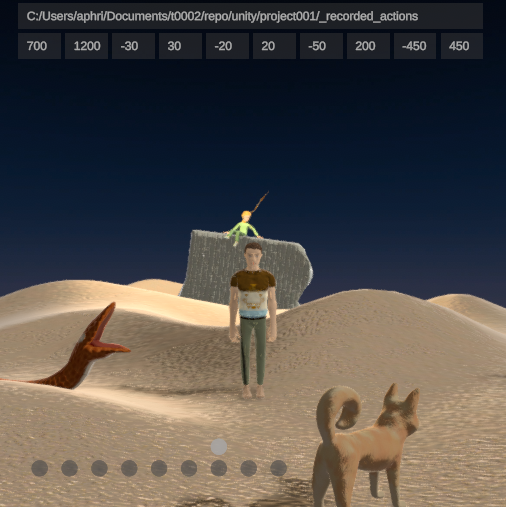
\includegraphics[width=\linewidth]{simulation_engine.png}
	\caption{Action simulation engine.}
	\label{fig:simulationengine}
\end{figure}

\subsection{Data Generation} Our data set is generated by a 3D simulation program(Figure \ref{fig:simulationengine}) developed in Unity that supports configurations for zoom, center offset, camera angle orientation and avatar styles. The amount of zoom applied to the camera typically varies from 50\% to 200\%, 100\% represents the default zoom amount. An offset could be applied to the x or y direction of the the camera relative to the target of the camera, the unit of this configuration is based on the simulation world space metric system (meters in world space).  The camera could also be rotated about the x and y axis relative to the target avatar, we typically set these configurations between -5 degrees to 90 degrees about the x axis and -90 degrees to 90 degrees about the y axis(Figure \ref{fig:orientationfig}).

\begin{figure}
	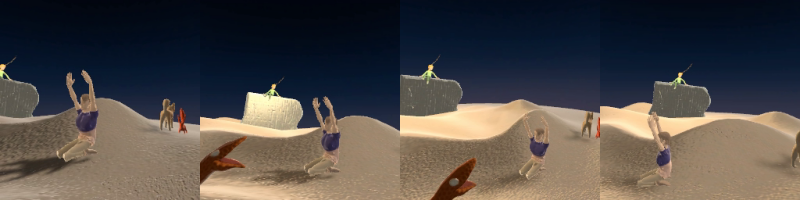
\includegraphics[width=\linewidth]{orientation_fig.png}
	\caption{Various camera angle, offset and zoom configurations.}
	\label{fig:orientationfig}
\end{figure}

\begin{figure}
	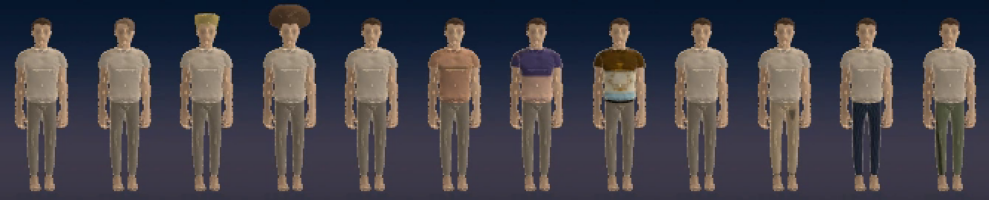
\includegraphics[width=\linewidth]{appearance_fig2.png}
	\caption{Appearance styles. First set of 4 figures show possible hairstyles. Second set of 4 figures show possible cloth patterns. Third set of 4 figures shows possible pants patterns.}
	\label{fig:appearancefig}
\end{figure}

The avatar character in the simulation could be configured with various hair, cloth and pants style. In our current iteration, there are 4 different styles for hair, cloth and pants respectively, for a total of 64 unique combinations(Figure \ref{fig:appearancefig}).

Our first set of actions include a total of 10 different yoga poses: camel, chair, childs, lord of the dance, lotus, thunderbolt, triangle, upward dog, warrior II and warrior III. Each of the 10 yoga poses have 4 type variations within them, some with more pronounced difference than others,  for a total of 40 action and action types(Figure \ref{fig:actionsfig}). We have decided to choose this set of actions as our first action sets because each pose is distinct and has a defined ending position, which allows us to use image classification techniques to compare classic modeling architecture and deep learning ones.

Our simulation also supports the option to include static background and dynamic background objects which would allow us to adjust the complexity of the sample data.

\subsection{Data Set} From the actions and configurations available within our simulation program, we generated 3 sets of video actions data of varying difficulties based on the zoom, offset, angle and scene background configurations specified: easy, medium and hard.

The configurations of the three datasets are listed in the Table \ref{tab:dataconfig}. Each dataset is generated as follows: for each of the 40 action and action types, we sample 25 random hair, cloth and pants style combinations to create action scenes for, and for each action scene, we capture the action with 20 cameras of randomly generated offsets and angles based on the constraints specified. Each dataset is therefore consisted of 20,000 videos, every action and action type label combination contains 500 videos and every action label contains 2000 videos. Figure \ref{fig:difficultylevels} shows samples from each difficulty level.

\begin{figure}
	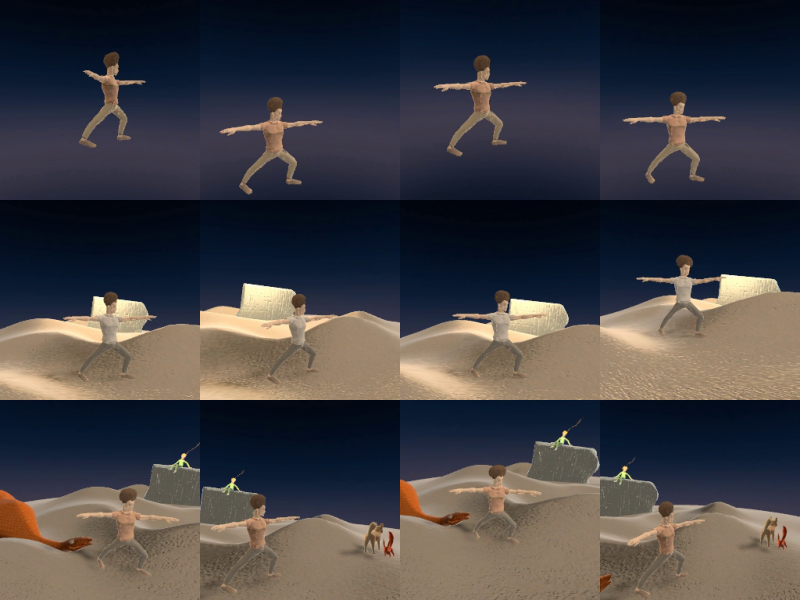
\includegraphics[width=\linewidth]{difficulty_levels.png}
	\caption{Difficulty levels. First row shows samples from easy level data set. Second row shows samples from medium level data set. Third row shows samples from hard level data set.}
	\label{fig:difficultylevels}
\end{figure}

\begin{table} % Single column table
	\caption{Data set configurations: zoom in percentage, offset in meters, angle in degrees.}
	\centering
	\begin{tabular}{lccc}
		\toprule
		Type & Easy & Medium & Hard  \\
		\midrule
		Min. Zoom & 80\% & 80\% & 70\% \\
		Max. Zoom & 110\% &  110\% & 120\%  \\
		\hline
		Min. X Offset & -1.5 & -1.5 & -3.0 \\
		Max. X Offset &  1.5 & 1.5 & 3.0 \\
		\hline
		Min. Y Offset & -1.5 & -1.5 & -2.0 \\
		Max. Y Offset &  1.5 & 1.5 & 2.0 \\
		\hline
		Min. X Angle & -5$^{\circ}$ & -5$^{\circ}$ & -5$^{\circ}$ \\
		Max. X Angle & 10$^{\circ}$ & 10$^{\circ}$ & 20$^{\circ}$ \\
		\hline
		Min. Y Angle & -30$^{\circ}$ & -30$^{\circ}$ & -45$^{\circ}$ \\
		Max. Y Angle & 30$^{\circ}$ & 30$^{\circ}$ & 45$^{\circ}$ \\
		\hline
		Static Background & Off & On & On \\
		Dynamic Background & Off & Off & On \\
		\bottomrule
	\end{tabular}
	\label{tab:dataconfig}
\end{table}

As we can see from Table \ref{tab:dataconfig}, the configuration of easy and medium dataset is identical except medium dataset has static background turned on.

Each video is typically about 1 second in length, sampled at 30 FPS. the size of each video is around 80KB and the frame is 351X351 pixels.

\section{Model}

For the modeling section of this research, we have extracted the frame at 50\% location of each video as input to our models, since the actions within each video are yoga poses and could be adequately represented by the middle frame. This approach would ideally be enhanced later to use multiple frames within each video, supplemented with temporal information represented by optical flow.

Each frame extracted from the video as 256X256X3 pixel RBG image, then converted to grayscale image of 256X256 pixels. Afterwards, we crop top, bottom, left and right of each grayscale image by 70, 30, 50 and 50 pixels to create 156X156 pixels grayscale image, in order to further reduce the size of input data.

\subsection{Filter}

\subsubsection{Principal Component Analysis} For computing PCA, we first downsize the input grayscale frame by 50\% to 78X78 pixels and flatten the image into an array of length 6084. Then we apply PCA on the input array, keeping the top 256 principal components. Finally each of the image array is projected onto the top 256 components to create the PCA weights for each image.

\subsubsection{Histogram of Oriented Gradients} In order to compute the HOG features, we first crop the input grayscale image to 100X100 pixels, due to the amount of time HOG computation requires. Then HOG feature descriptor is computed with 9 orientations, 2x2 pixels per cell and 2x2 cells per block.

\subsubsection{Scale-Invariant feature transform} Bag of Words is a commonly used technique in image classification. Similar to NLP, image features are used as words. We utilized SIFT features for this purpose. SIFT is one of the important algorithms that detect objects irrelevant to the scale and rotation of the image and the reference. This helps a lot while we are comparing the real-world objects to an image though it is independent of the angle and scale of the image.
We used OpenCV to extract SIFT descriptors for each image.The descriptors were clustered into N (N=60) number of clusters. Then a feature vector v \in \(\mathbb{R}\) ^n   was built where each direction represented a cluster and magnitude represented the count of SIFT descriptors in that cluster for the image.


\subsection{Classifier}

\subsubsection{Support Vector Machine} We use the support vector classification directly from Scikit-Learn with the default parameters: 1.0 for regularization, radial basis function as kernel and maximum iterations of 50. 

\subsubsection{Logistic Regression} Again we use the logistic regression function from Scikit-Learn with default parameters: ``LBFGS'' as the solver and maximum iterations of 100.

\subsubsection{Gradient Boosting Tree} The gradient boosting tree we trained uses 100 estimators, each with a maximum depth of 3 and a learning rate of 0.1.

\subsubsection{Convolutional Neural Network}  Our convolutional neural network model is inspired by the VGG-16 CNN model. The model consists of 10 convolutional layers, where the first two layers extract 32 features and subequent pairs of layers extract double the number of features from the previous layers. After each pair of layers, a max pooling of size 2X2 is applied to the input features from the previous convolutional layers. Finally, two dense layers followed by a classification layer is applied to generate the model prediction. 

\section{Evaluation}

\subsection{Baseline}

Our baseline for evaluation is the SVM model trained on the unfiltered input data scaled down to 20\% at the ``easy'' level. We felt that this model is the most natural starting point to evaluate how effective the various types of filtering and modeling techniques are and how much they contribute to the final accuracy of the models.

\subsection{Process}

We start out by training our baseline models on the ``easy'' level dataset, which produces a guideline for choosing models for further training. Then combinations of filters and models with the best results are trained on the ``medium'' level dataset to assess the capabilities of the models. Finally the best performance models are challenged with the ``hard'' dataset for evaluation.

For every data set and model training, we split the sample data into three sets, training set, validation set and test set, in the ratio of 8:1:1. For classic models, validation data set is not used at all, training set is used to train and optionally validate during training depending on the model in question (GBT), and test data set is used to compute the final accuracy of the models.

\section{Results}

\begin{table*} % Full width table (notice the starred environment)
	\caption{Model results for each difficulty level and model/filter combination. Action column displays results for using action only as label, A+T column displays results for using action and action type combination as label.  }
	\centering % Horizontally center the table
	\begin{tabular}{L{0.1\linewidth} L{0.1\linewidth} C{0.05\linewidth} C{0.05\linewidth} C{0.05\linewidth} C{0.05\linewidth} C{0.05\linewidth} C{0.05\linewidth} C{0.05\linewidth} C{0.05\linewidth}}
		\toprule
		\multicolumn{2}{c}{} & \multicolumn{2}{c}{Easy} & \multicolumn{2}{c}{Medium} & \multicolumn{2}{c}{Hard}\\
		\cmidrule(r){3-8}
		Model & Filter & Action & A+T & Action & A+T & Action & A+T \\
		\midrule
		SVM & Downsize & 37\% & 29\% & 15\% & 5\% & - & - \\
		Logistic & Downsize & 43\% & 16\% & 21\% & 6\% & - & - \\
		GBT & Downsize & 71\% & 29\% & 61\% & 14\% & - & - \\
		\hline
		SVM & PCA & 48\% & 42\% & 15\% & 6\% & - & - \\
		Logistic & PCA & 44\% & 17\% & 23\% & 6\% & - & - \\
		GBT & PCA & 69\% & 30\% & 24\% & 3\% & - & - \\
		\hline
		SVM & HOG|PCA & 68\% & 54\% & 27\% & 11\% & - & - \\
		Logistic & HOG|PCA & 55\% & 21\% & 34\% & 10\% & - & - \\
		GBT & HOG|PCA & 85\% & 46\% & 30\% & 5\% & - & - \\
		\hline
		SVM & SIFT & 50\% & 43\% & 34\% & 28\% & 16\% & 9\% \\ 
   	   	Logistic & SIFT & 70\% & 46\% & 53\% & 30\% & 33\% & 13\% \\
   	   	GBT & SIFT & 71\% & 44\% & 56\% & 27\% & 32\% & 12\% \\ 
		\hline
		CNN & - & - & - & 100\% & 98\% & 95\% & 92\% \\
		\bottomrule
	\end{tabular}
	\label{tab:modelres}
\end{table*}

Table \ref{tab:modelres} shows the results from training and testing combinations of 4 models and 3 filters. We start out with the easy level data set, training 3 models (SVM, Logistic, GBT) with no filters except downsizing the input images by a further 80\%. The results show that gradient boosting tree generates the best performance out of the three models. However the results of SVM and GBT are comparable with action and action type label combination. Three more sets of models are trained on the easy level data set with the PCA filter, the HOG plus PCA filter combination and the SIFT filter. The results show steady improvements, where HOG plus PCA filter with SVM model achieving the best accuracy for action plus action type labels, although the SIFT filtered models perform better on average.

For the medium set, again we perform the same training and testing for all of the classic models, but this time also including the CNN model. As shown in the table, the CNN model easily outperforms all other models, achieving 98\% accuracy on the action plus action type labels. Second best performing models are the SIFT feature based models, achieving 28\% accuracy on average for action plus action type labels.



\section{Model Analysis}

placeholder

\section{Discussion}

placeholder

\section{Future}

placeholder

%----------------------------------------------------------------------------------------
%	 REFERENCES
%----------------------------------------------------------------------------------------

\phantomsection
\bibliographystyle{unsrt}
\bibliography{t0004.bib}

%----------------------------------------------------------------------------------------

\begin{figure*}
	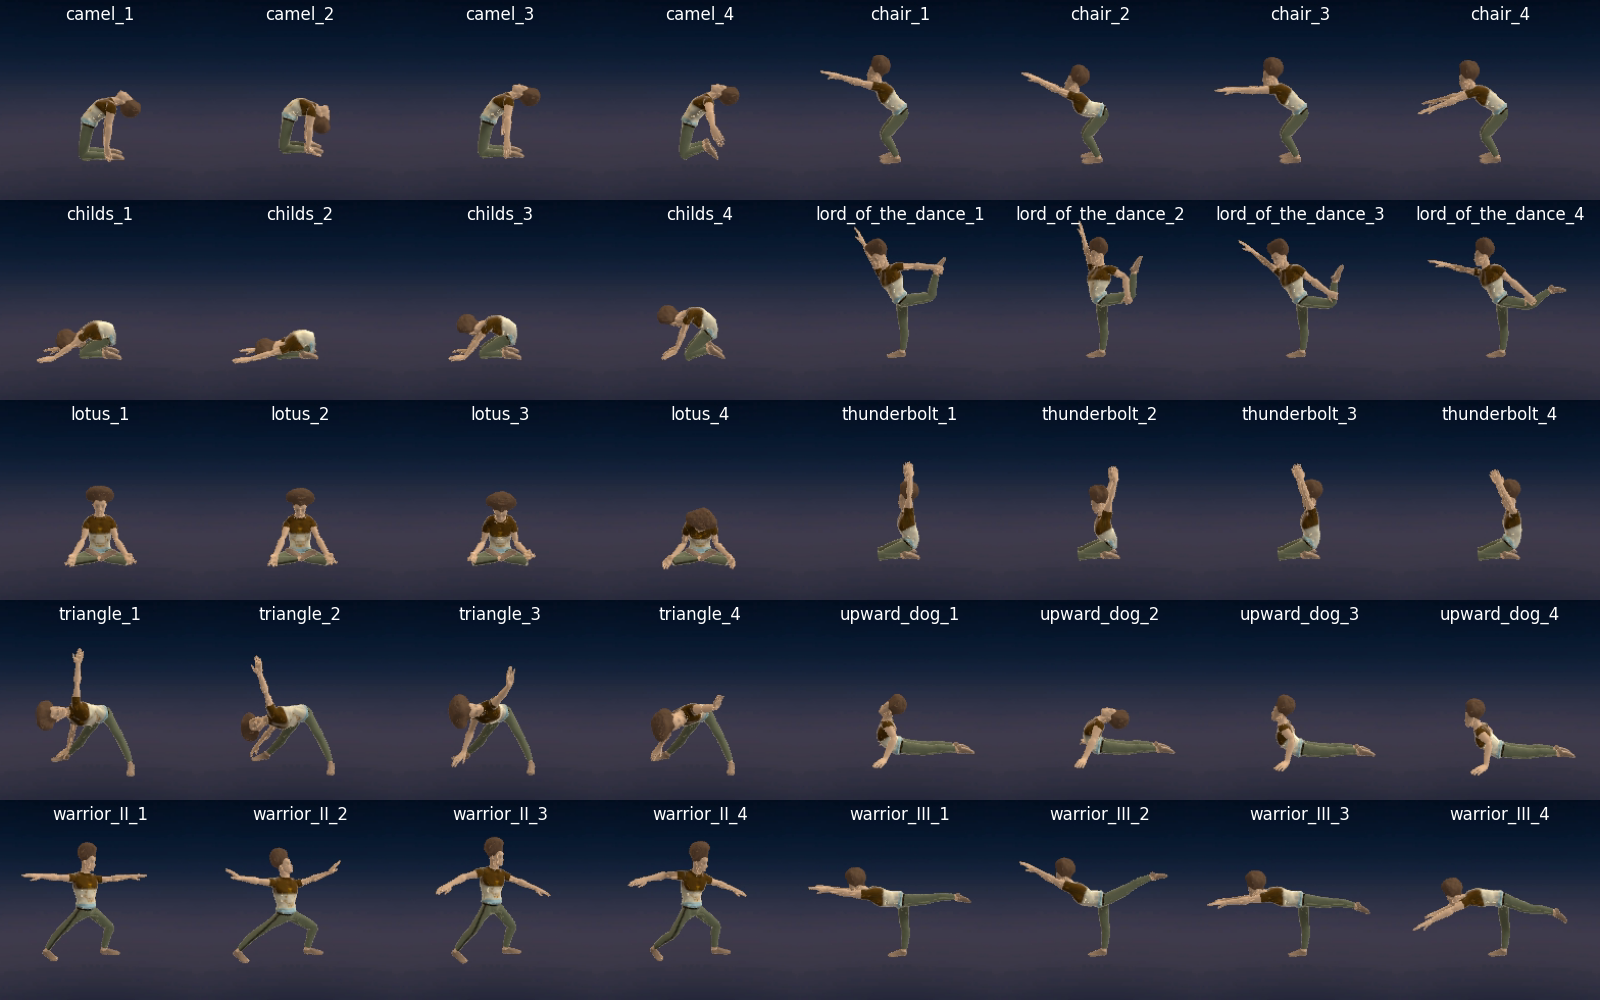
\includegraphics[width=\linewidth]{actions_fig.png}
	\caption{10 yoga poses, each with 4 different variaionts.}
	\label{fig:actionsfig}
\end{figure*}

\end{document}
